\documentclass[pdf]{article}
\usepackage{pst-node}
\usepackage{amssymb}

\usepackage{tikz-cd} 
\usepackage{amsmath}
\usepackage{amsthm}
\usepackage{pgfplots}
\pgfplotsset{width=10cm,compat=1.9}
\usepackage{graphicx} %package to manage images
\usepackage{hyperref}

\newcommand{\vect}[1]{\boldsymbol{#1}}
\newtheorem{theorem}{Theorem}[section]
\newtheorem{corollary}{Corollary}[theorem]
\newtheorem{lemma}[theorem]{Lemma}
\newtheorem{note}[theorem]{Note}
\newtheorem{subnote}[corollary]{Sub-Note}
\newtheorem{myQuestion}[theorem]{My-Question}
\newtheorem{problem}[corollary]{Problem}


\begin{document}

\section{Cayley-Hamilton Theorem Revisit}

\subsection{Question}
Let's define a block determinate $det_n k^{nm\times nm} \to k^{n\times n}$, for any block matrix $M = [M_{ij}]_{1\leq i, j, \leq m}$, with $M_{ij}\in k^{n\times n}$,
\begin{align*}
det_n(M) = \sum\limits_\sigma (-1)^{sgn(\sigma)}\Pi_{i=1}^mM_{i\sigma(i)}
\end{align*}
Let $A$, $B$ be $n\times n$ matrices, lets define $n^2\times n^2$ matrices:
\begin{align*}
F(A,B) &= [a_{ij}B]_{1\leq i, j \leq n}\\
F(B,A) &= [b_{ij}A]_{1\leq i, j \leq n}
\end{align*}
Then Cayley-Hamilton states that $det_n(F(A,I_n) - F(I_n,A)) = 0_{n\times n}$.\\
\begin{myQuestion}\label{general_CH_Thm}
Is it true that $det_n(F(A,B) - F(B,A)) = 0_{n\times n}$, for any commutable $n\times n$ matrix $A$ and $B$, i.e. $AB=BA$?
\end{myQuestion}
\begin{note}
	Can start with looking at complex matrces, and for complex matrix, it may be suffice to study the cases for $B$ is a diagonal matrix.
	\begin{proof}[Answer is Yes for complex matrces if $B$ is diagonalizable]
		If $B$ is a diagonal and blockwise scaler matrix, i.e. $B =  diag\{B_1, B_2, \cdots, B_p\}$, and $B_i = b_i I_{n_i}$ for $i\in 1,\cdots,p$, then because $AB=BA$ $A$ is also block diagonal $A = diag\{A_1,\cdots,A_p\}$. Lets denote $f_i(x)$ to be the eigen polynomial of $A_i$, then 
	\begin{align*}
		det_n(F(B,A) - F(A,B) ) &= \Pi_{i=1}^pf_i(A)b_i^{n_i}\\
					      &= \Pi_{i=1}^pb_i^{n_i}\Pi_{i=1}^pf_i(A)\\
					      &= \det(B)\Pi_{i=1}^p diag\{f_i(A_j)\}_{j=1}^p\\
					      &= \det(B) diag\{\Pi_{i=1}^pf_i(A_j)\}_{j=1}^p
	\end{align*}
	Cayley-Hamilton theorem shows that $f_j(A_j) = 0_{n\times n}$, therefore $\Pi_{i=1}^pf_i(A_j) = 0_{n_j\times n_j}$ for each $j$. So we have
	\begin{align*}
		det_n(F(B,A) - F(A,B) ) &= \det(B) diag\{\Pi_{i=1}^pf_i(A_j)\}_{j=1}^p\\
					      &= \det(B) diag\{0_{n_j\times n_j}\}_{j=1}^p\\
					      &= \det(B) 0_{n\times n}\\
					      &= 0_{n\times n}\\
	\end{align*}
	\end{proof}
\end{note}

\begin{note}[Answer to Question \ref{general_CH_Thm} (20210401)]
After reading a very good interpretation of proof of Cayley-Hamilton Thoerem from \href{https://www.zhihu.com/question/57468352/answer/153402620}{How to understand the proof of Cayley-Hamilton Thoerem}. We can prove that $det_n(F(A,B^T) - F(B,A^T)) = 0_{n\times n}$, instead of $det_n(F(A,B) - F(B,A)) = 0_{n\times n}$. But I have already showed that if $B$ is diagonalizable then $det_n(F(A,B) - F(B,A)) = 0_{n\times n}$. In fact it is not hard to show that when $B=I$, $$det_n(F(A,B^T) - F(B,A^T)) = det_n(F(A,B) - F(B,A))$$, but is this true for general $B$?
\end{note}

\subsection{They Journal to Jordan form of complex Matrix}\label{Eigen-Value}

\begin{lemma}
For complex matrix $A$, and complex polynomia $p(t)$, then for any eigen-value $\lambda$ of $p(A)$, there exist eigen-value $\mu$ of $A$, such that $p(\mu) = \lambda$.
\end{lemma}
\begin{proof}
	Let $v$ be a eigen vector of $p(A)$ and $p(A)v = \lambda v$. We denote $q(x) = p(x) - \lambda$, then $q(A)v = 0$. Because $q(x) \in \mathbb{C}[x]$, it has a decomposition $q(x) = \Pi_{i=1}^n(x-\mu_i)$. Therefore we have
		\begin{align*}
		\Pi_{i=1}^n(A-\mu_i I_n)v = 0
		\end{align*}
	If we define $s_k = \Pi_{i=1}^k(A-\mu_i I_n)v$, where $k\in\{1, \cdots, n\}$. It is by definition that $s_n = 0$, and $s_0 != 0$. Let $0<m\leq n$ be the smallest interger with $s_m = 0$, then 
		\begin{align*}
		0= s_m = \Pi_{i=1}^m(A-\mu_i I_n)v = (A-\mu_m I_n)s_{m-1} = As_{m-1} - \mu_ms_{m-1}
		\end{align*}
	This gives that for non-zero vector $s_{m-1}$
		\begin{align*}
		As_{m-1} = \mu_ms_{m-1}
		\end{align*}
	So $\mu_m$ is an eigen-vector of $A$, and $\mu_m$ is a root of $q(x)$, i.e. $p(\mu_m) = \lambda$.
\end{proof}

\begin{note}
This result is not nessesary correct for non-algebraic close field. For example:
\begin{align*}
A = \begin{bmatrix}
0 & 1\\
-1 & 0
\end{bmatrix}
\end{align*}
Then $A^2 = -I_2$. so $A^2$ has eigen value $-1$, but $A$ don't have any real eigen value.
\end{note}

\section{Triangular Function}
Triangular functions $\sin$, $\cos$ has the following formulas:
\begin{align*}
\sin(\alpha + \beta) &= \sin(\alpha)\cos(\beta) + \sin(\beta)\cos(\alpha)\\
\sin(\alpha - \beta) &= \sin(\alpha)\cos(\beta) - \sin(\beta)\cos(\alpha)\\
\cos(\alpha + \beta) &= \cos(\alpha)\cos(\beta) - \sin(\beta)\sin(\alpha)\\
\cos(\alpha - \beta) &= \cos(\alpha)\cos(\beta) + \sin(\beta)\sin(\alpha)
\end{align*}
\subsection{Question}
What if we define functions, replacing the right angle by an angle of size $A$.
\begin{align*}
S_A(\alpha) &= \sin(\alpha)/\sin(A)\\
C_A(\alpha) &= S_A(\pi - A - \alpha)
\end{align*}
Then we can prove that half of the above trig-formulas are still valid, while others are not!!
\begin{align*}
C_A(\alpha + \beta) &= C_A(\alpha)C_A(\beta) - S_A(\beta)S_A(\alpha)\\
S_A(\alpha - \beta) &= S_A(\alpha)C_A(\beta) - S_A(\beta)C_A(\alpha)
C_A(\alpha - \beta) &= C_A(\alpha)C_A(\beta) + S_A(\beta)S_A(\alpha)
\end{align*}
\begin{align*}
S_A(\alpha + \beta) &= S_A(\alpha)C_A(\beta) + S_A(\beta)C_A(\alpha) - 2S_A(\alpha)S_A(\beta)\cos(A)\\
\end{align*}
For example:
\begin{align*}
C_A(\alpha) &= S_A(\pi - A - \alpha)\\
                    &= \sin(\pi - A - \alpha)/\sin(A)\\
                    &= \sin(\pi/2 + \pi/2 - A - \alpha)/\sin(A)\\
                    &= \sin(\pi/2 - (\alpha - (\pi/2 - A)))/\sin(A)\\
                    &= \cos(\alpha - (\pi/2 - A))/\sin(A)\\
                    &= ( \cos(\alpha)\cos((\pi/2 - A)) + \sin(\alpha)\sin((\pi/2 - A)) )/\sin(A)\\
                    &= ( \cos(\alpha)\sin(A) + \sin(\alpha)\cos(A) )/\sin(A)\\
                    &= \cos(\alpha) + S_A(\alpha)\cos(A)
\end{align*}
which means,
\begin{align*}
\cos(\alpha) = C_A(\alpha) - S_A(\alpha)\cos(A)
\end{align*}
Therefore,
\begin{align*}
S_A(\alpha + \beta) &= \sin(\alpha + \beta)/\sin(A)\\
			 &= (\sin(\alpha)\cos(\beta) + \sin(\beta)\cos(\alpha))/\sin(A)\\
			 &= (S_A(\alpha)\cos(\beta) + S_A(\beta)\cos(\alpha))\\
			 &= S_A(\alpha)(C_A(\beta) - S_A(\beta)\cos(A)) + S_A(\beta)(C_A(\alpha) - S_A(\alpha)\cos(A))\\
			 &= S_A(\alpha)C_A(\beta) + S_A(\beta)C_A(\alpha)
\end{align*}
\begin{myQuestion}
if the trig-formulas do not strictly require $A = \pi/2$, then what is the reason behand the trig-functions? How about the Taylor expansion of $S_A(x)$ and $C_S(x)$? Do we get any interesting things about calculating $\pi$?
\end{myQuestion}
\begin{lemma}[Proof using triangle areas] Lets think about the following three line segments $OA$, $OB$, $OC$. Then $$\bigtriangleup OAB + \bigtriangleup OBC = \frac{1}{2}(|BA||BO|\sin(\Gamma) + |BO||BC|\sin(\Gamma))$$
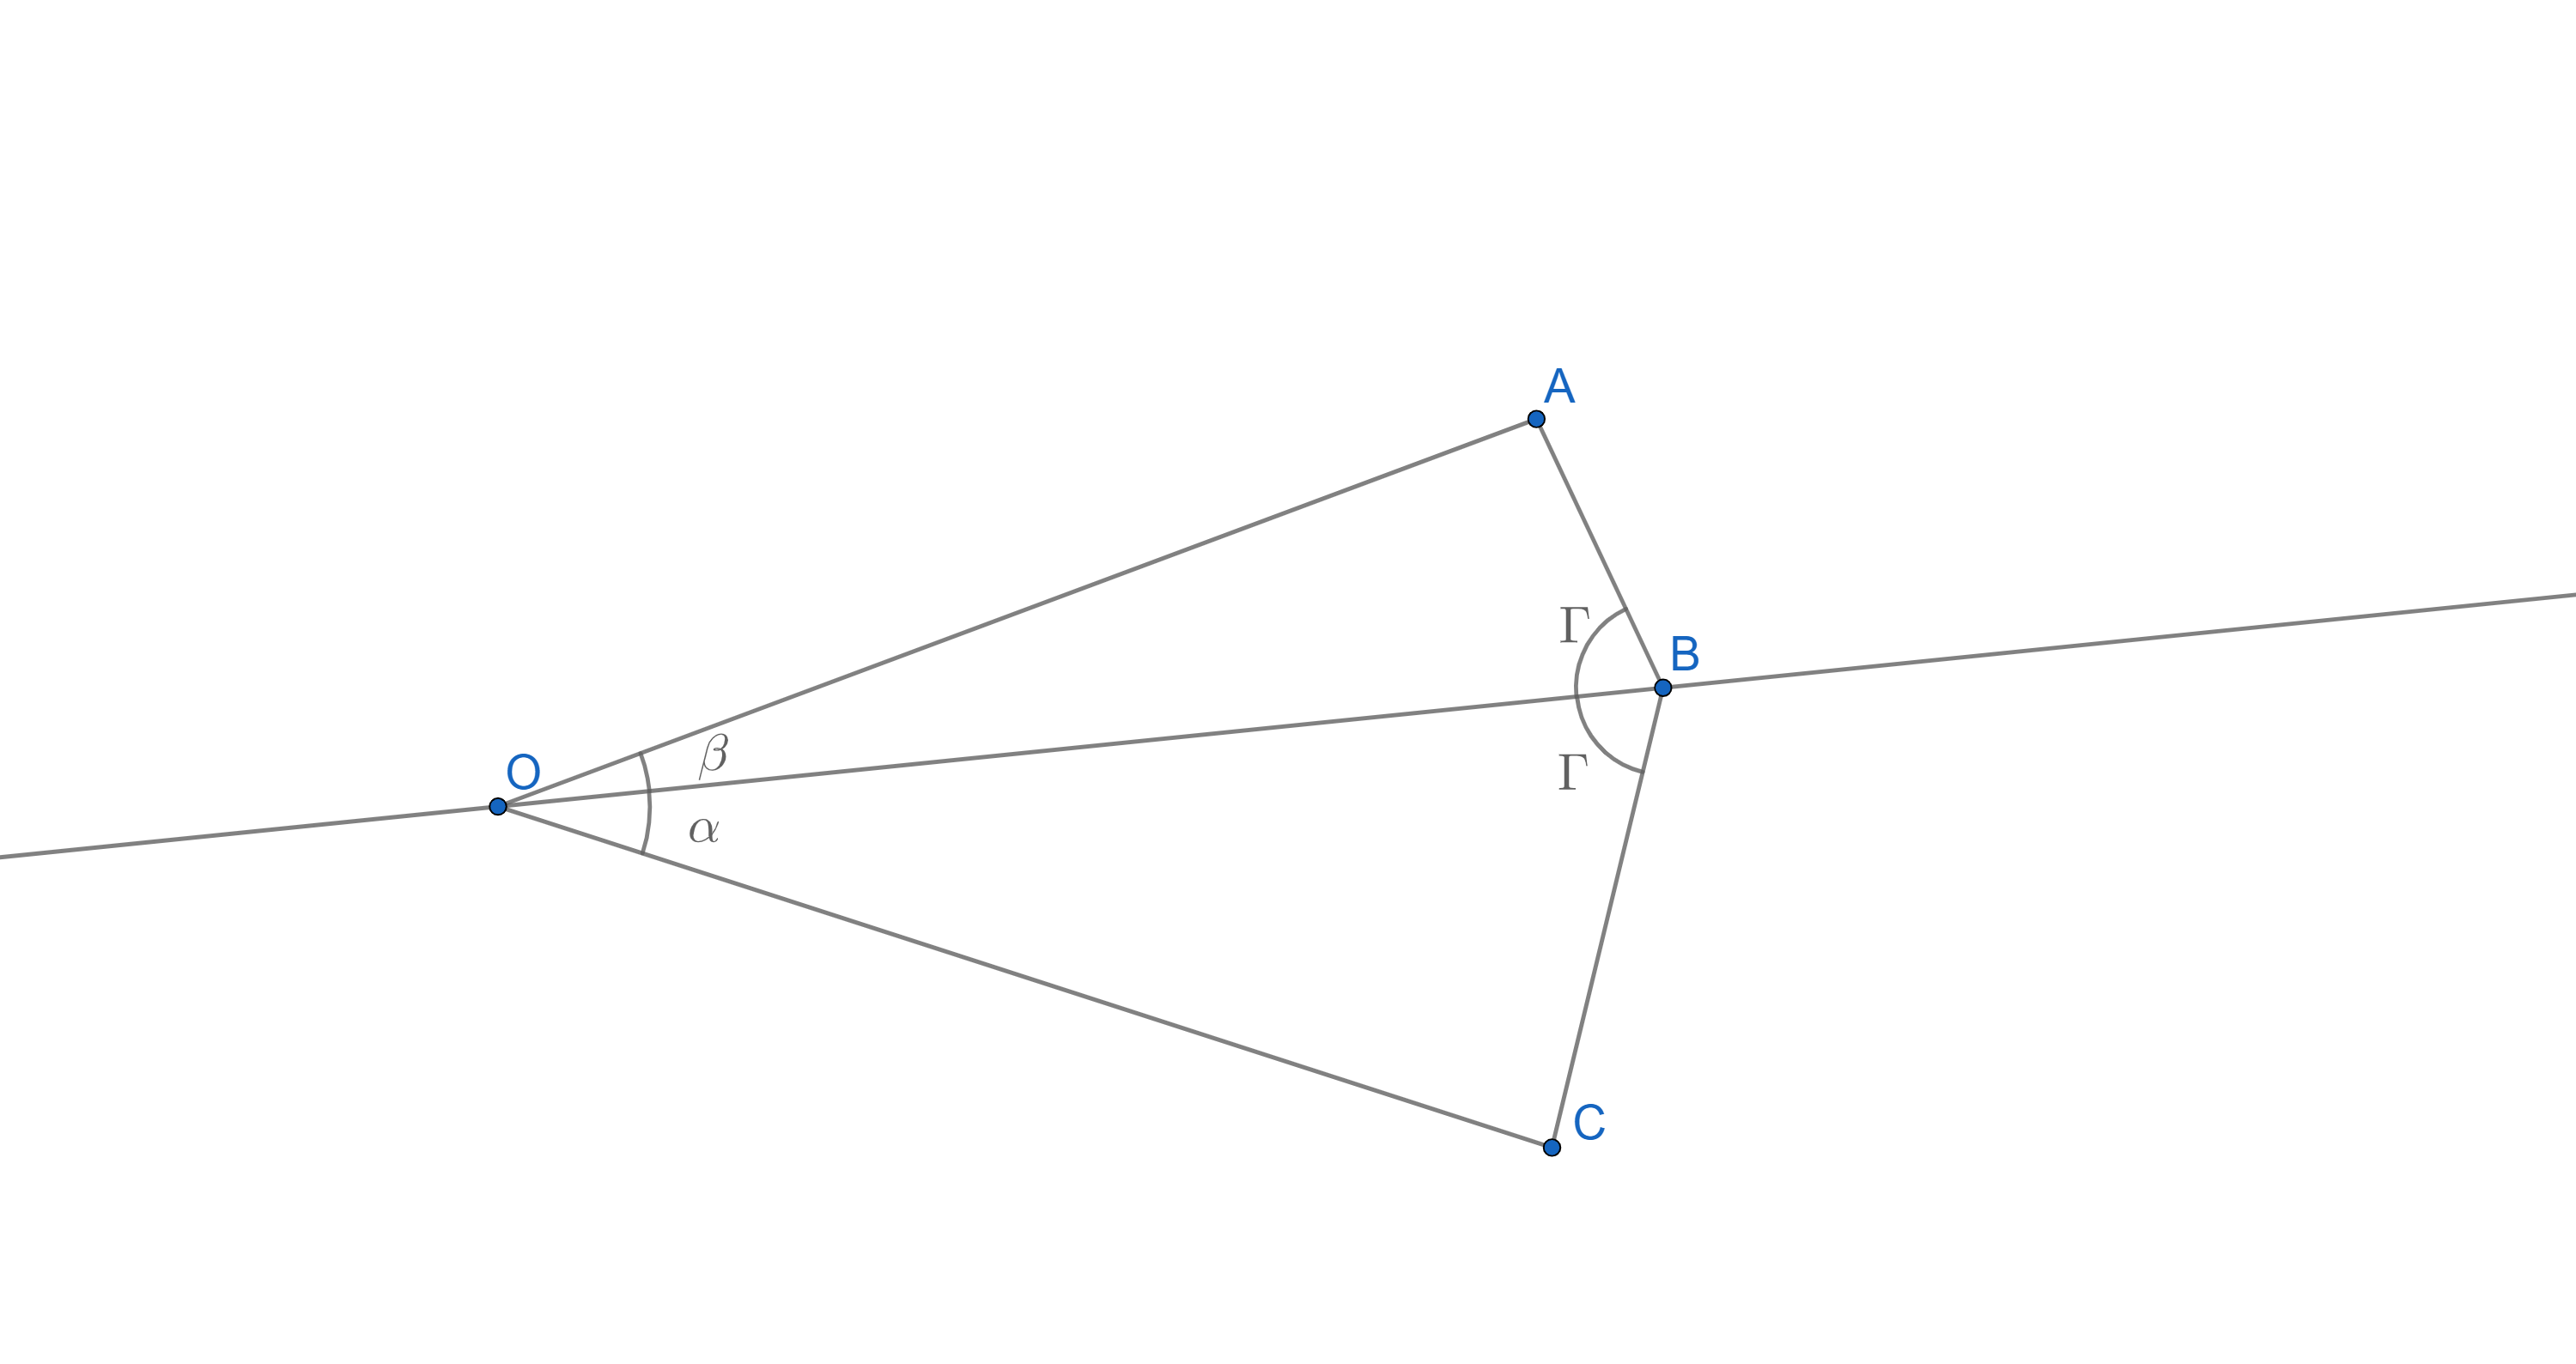
\includegraphics{trig_formula_graph_1}

\end{lemma}

\section{Triangular Formula}
I was  trying to find a simple proof of triangular formula $$\sin(\alpha+\beta) = \sin\alpha\cos\beta + \cos\alpha\sin\beta.$$ One idea is to use $e^{i\theta} = \cos\theta + i\sin\theta$, and $e^{i(\alpha + \beta)} = e^{i\alpha} \cdot e^{i\beta}$. The Euler formula is not trivial, so it can not serve as a valid proof, but it does give a path to the proof.\\

Consider maps $P_{\theta}: \mathbb{C}\to\mathbb{C}$, with $P_\theta(z) = (\cos\theta + i\sin\theta) \cdot z$. Then it is clear that:
\begin{itemize}
\item $P_{\theta}$ is a linear map.
\item $P_{\theta}$ on $1$ and $i$ are both rotation counter clockwise by $\theta$.
\end{itemize}
Therefore $P_{\theta}$ is a rotation of the whole plane by $\theta$. Now consider $z_\alpha = \cos\alpha + i\sin\alpha$, then we know that $P_\theta(z_\alpha) = z_{\alpha + \theta}$, in which,
\begin{align*}
z_{\alpha + \theta} &= \cos(\theta+\alpha) + i\sin(\theta+\alpha)\\
P_\theta(z_\alpha)  &= (\cos\theta + i\sin\theta)\cdot (\cos\alpha + i\sin\alpha)\\
&= (\cos\theta\cos\alpha  - \sin\theta\sin\alpha) + i(\sin\theta\cos\alpha  + \sin\alpha\cos\theta)
\end{align*}
So we get the two triangular formulas
\begin{align*}
\sin(\alpha+\beta) &= \sin\alpha\cos\beta + \cos\alpha\sin\beta\\
\cos(\alpha+\beta) &= \cos\alpha\cos\beta - \sin\alpha\sin\beta
\end{align*}
The concept of rotation is foudamental in geometry, and the concept of linear map is also foundamental. So the above should serve as a valid proof. And the follow graph can translate the above proof to the language of middle school geometry.\\
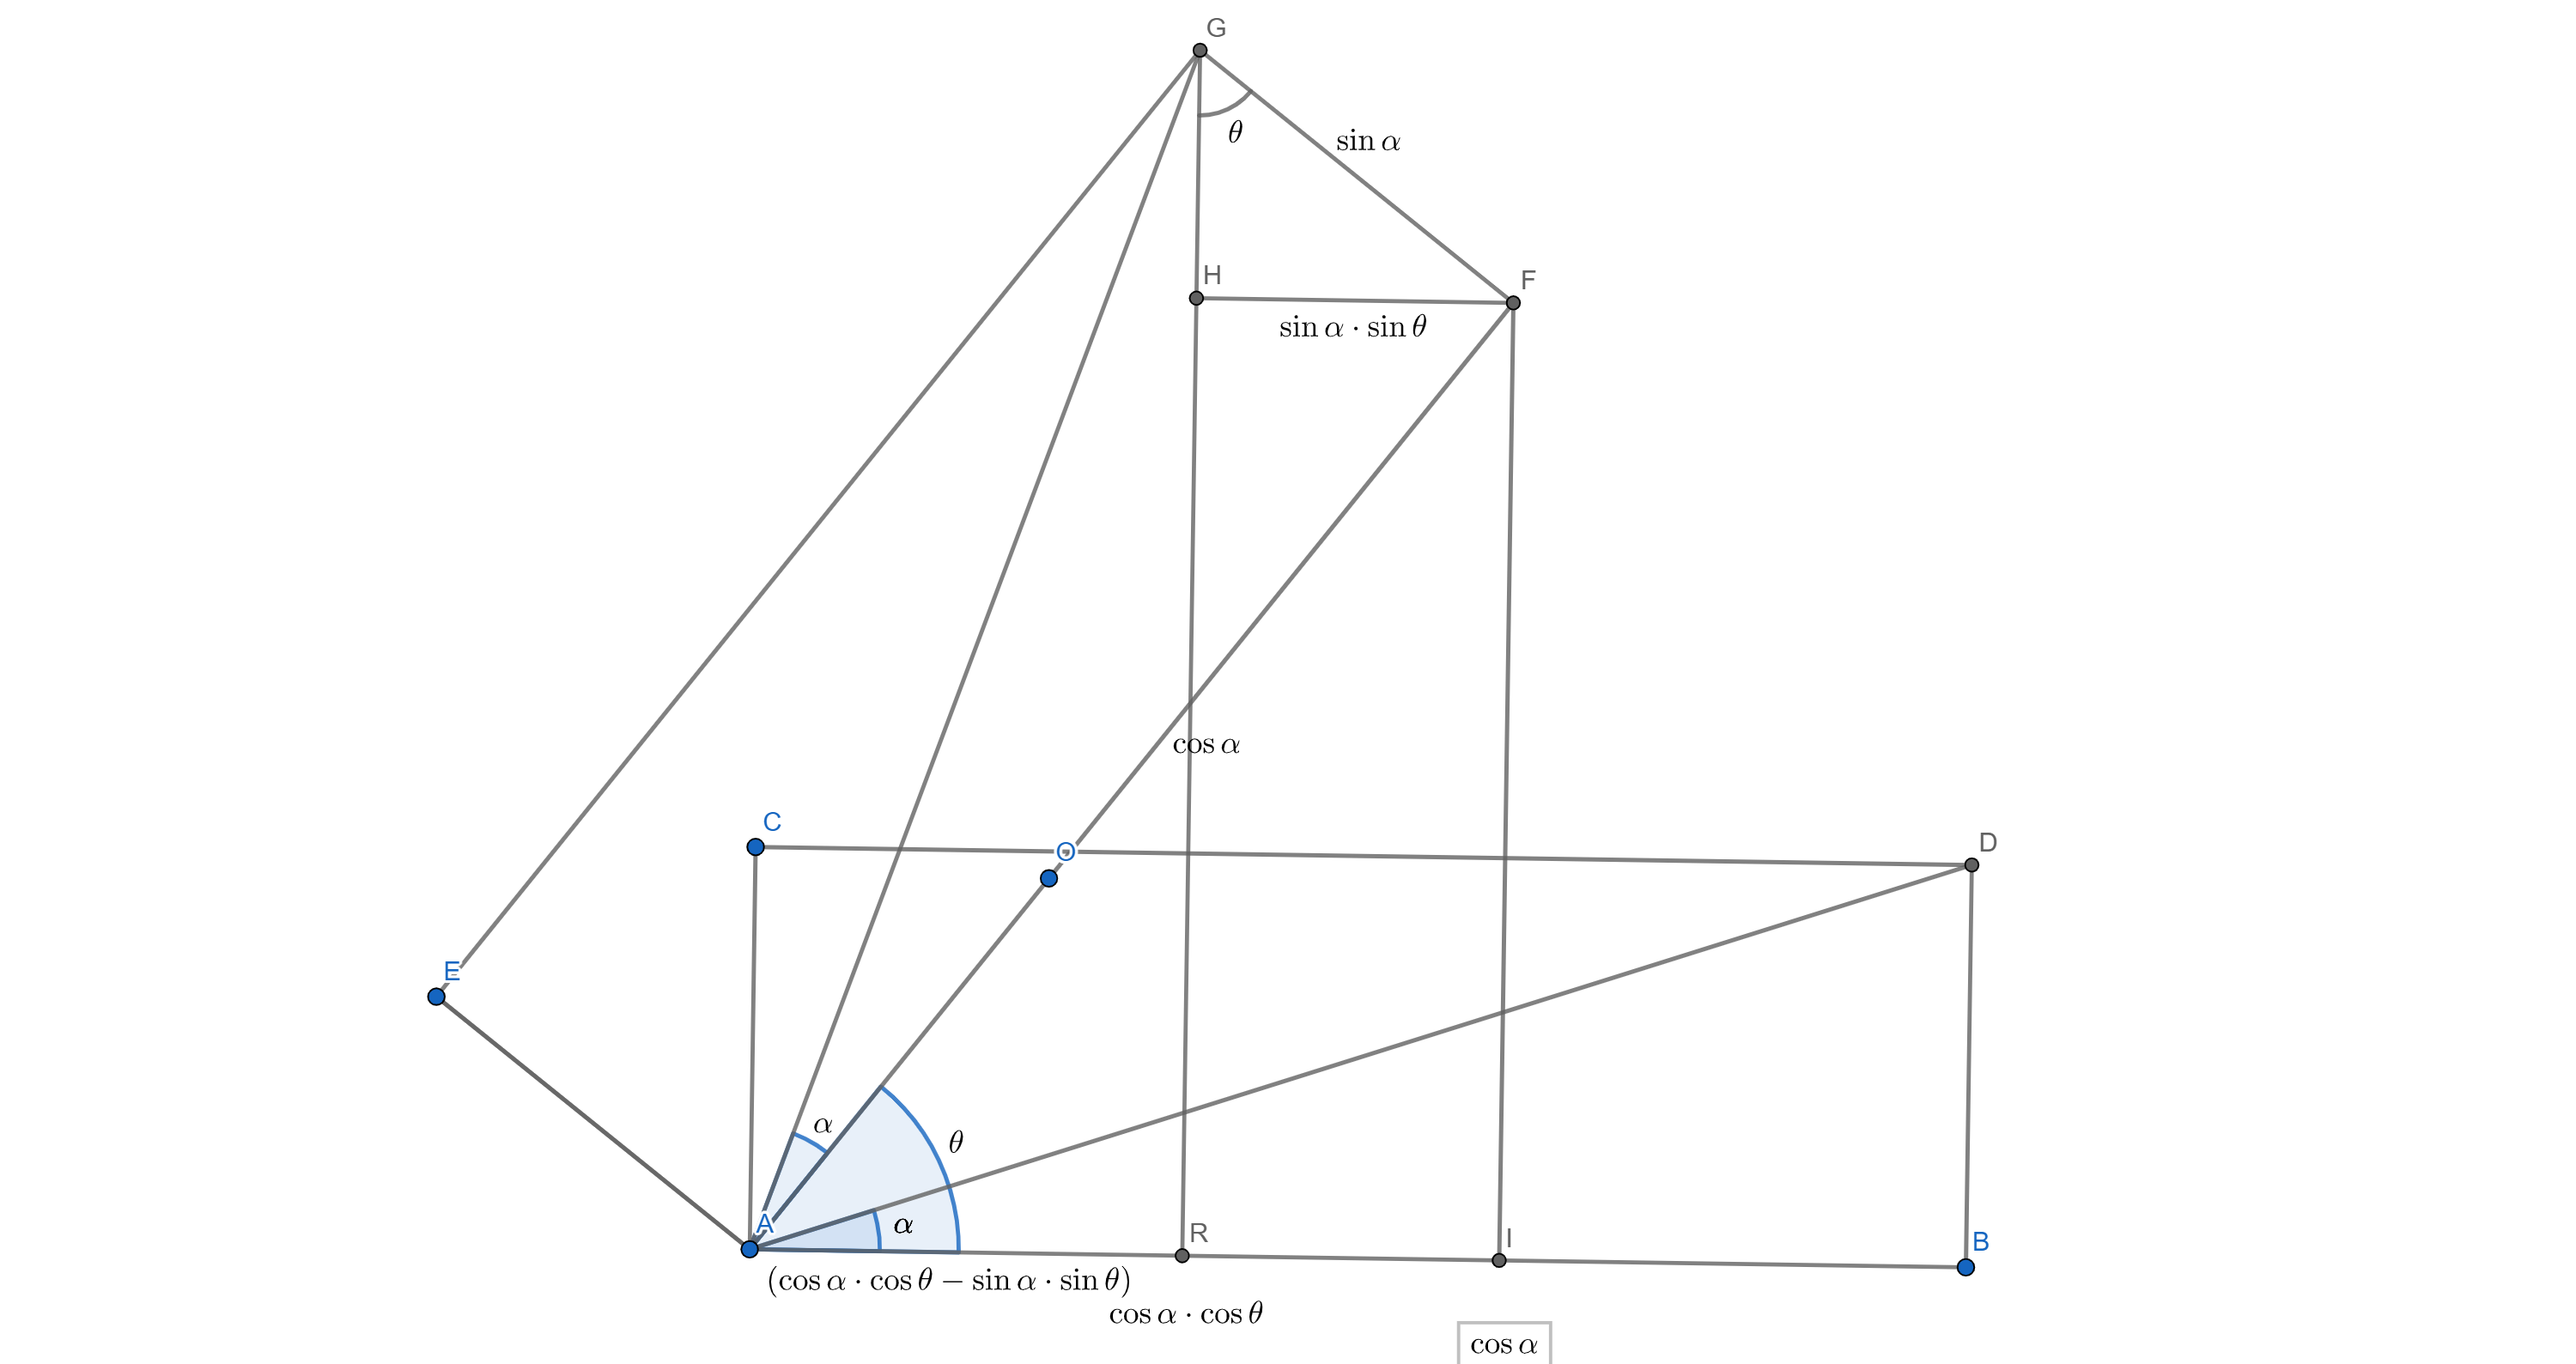
\includegraphics{triangular_formula}
One interesting observation here is that: triangular formulas don't require the pythagorean theorem, in particular, we don't need to use $\cos\theta^2 + \sin\theta^2 = 1.$

\section{Real Random Though}
\subsection{Quantum computing, neural network, consciousness, probability theory}
\begin{itemize}
\item How quantum computing can help Machine Learning?
\item How quantum mechenics can help explaining consciousness?
\item How Neural network is helping modeling brain?
\item whether quantum algorithm is better than classical algorithm? Can quantum computer be simulatable by classical computer?
\item P = NP ?
\item do we need new formulation of probability theory for better understanding of all above?
\end{itemize}



\end{document} 